\documentclass{article}
\usepackage[utf8]{inputenc}
\usepackage[utf8]{vietnam}
\usepackage{enumitem}
\usepackage{amsmath}
\usepackage{amsfonts}
\usepackage{amssymb}
\usepackage{amsthm}
%chèn gói hình ảnh

\newtheorem{lemma}{Bổ đề}
\newtheorem{theorem}{Định lý}
\newtheorem{proposition}{Bài}
%tạo evirontment cho Bài tập, có lựa chọn tên bài tập, chú thích trong ()
%ví dụ như Bài tập 3. (bài tập mô hình hóa - mở đầu)
\newenvironment{exercise}[2]{
     \setlength\parindent{0pt}\par\medskip\textbf{Bài tập #1. (#2)} \quad}{%
     \hfill\tiny$\blacksquare$\par\medskip}
%tạo environment cho bài toán, có lựa chọn lùi 3cm
\newenvironment{problem}[1]{%
     \setlength\parindent{#1 pt}\par\medskip\textbf{Bài toán.}}{}
\newenvironment{solution}{%
     \setlength\parindent{0pt}\par\medskip\textbf{Lời giải.}\quad}{%
     \hfill\tiny$\blacksquare$\par\medskip}
\newenvironment{answer}{%
     \setlength\parindent{0pt}\par\medskip\textbf{-}\quad}{}
\newenvironment{constraint}{%
     \setlength\parindent{0pt}\par\medskip\textbf{Điều kiện.}\quad}{%
     }
\usepackage[left=2cm,right=2cm,top=2cm,bottom=2cm]{geometry}
\setlength{\parindent}{0pt}
%chèn file.pdf
\usepackage{graphicx}
\usepackage{caption}
%làm sao chèn file pdf vào latex
\usepackage{pdfpages}
\begin{document}
%chen đoạn pdf
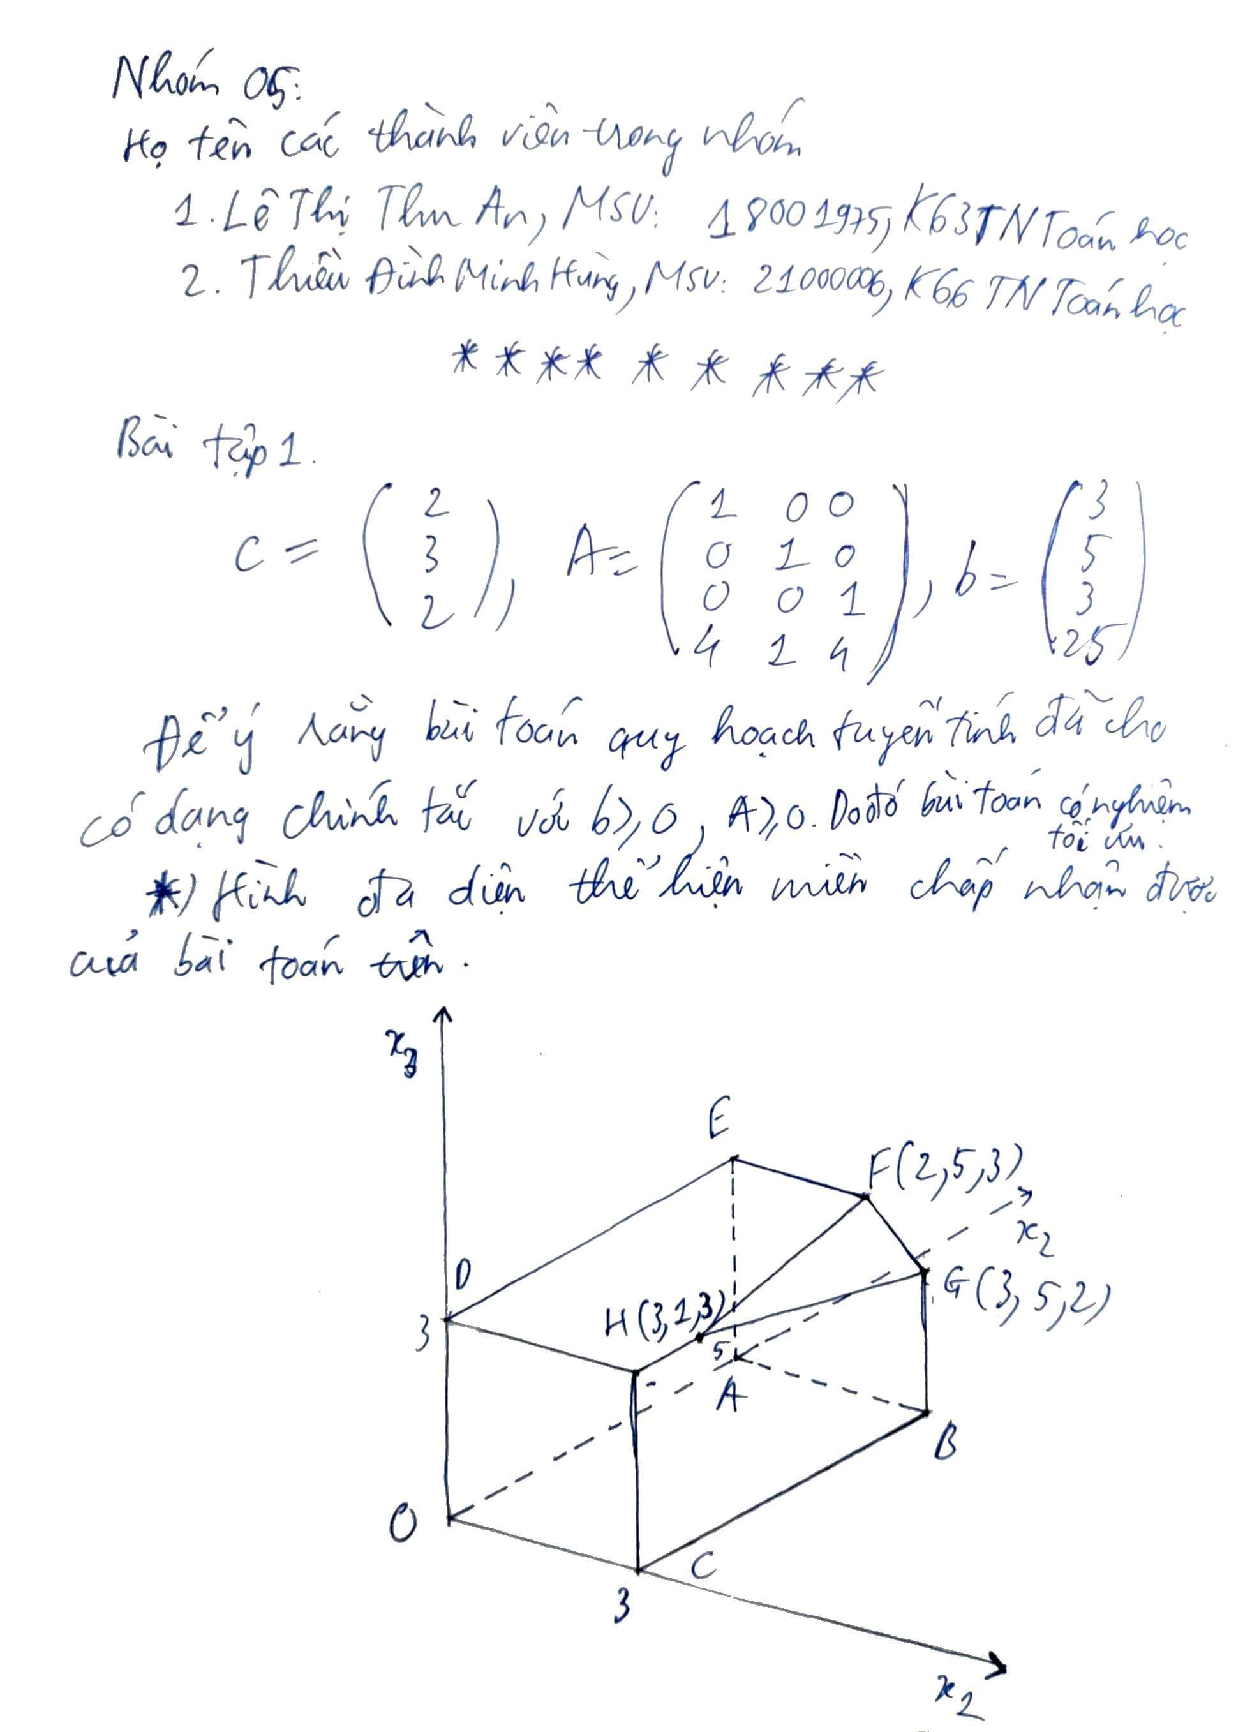
\includepdf[pages=-]{Bai 1}

%Bài tập 3. (bài tập mô hình hóa - mở đầu)
%Nhóm 5
%Bài 3. (bài tập mô hình hóa - mở đầu)
\begin{exercise}{3}{Bài tập mô hình hóa - mở đầu}

    Xét một bài toán nổi tiếng:
    %lùi 3cm

    \begin{problem}{10}
        Đặt nhiều quân hậu trên bàn cờ vua tiêu chuẩn 8 × 8 nhất có thể sao cho
không có hai quân hậu nào tấn công nhau.
    \end{problem}
    \begin{solution}
    Bàn cờ vua tiêu chuẩn có 8 hàng và 8 cột. Ta định nghĩa một đường chéo là một tập hợp gồm ít
    nhất hai tọa độ, các tọa độ cùng nằm trên một đường thẳng tọa với trục ngang (cũng như trục
    dọc) một góc $45$ độ. Có tất cả 26 đường chéo trên bàn cờ vua. Một quân hậu có thể tấn công
    một quân khác trên một ô cùng hàng ngang, cột dọc, hoặc đường chéo nếu những ô ở giữa là trống.

    Ta sẽ xây dựng một mô hình tối ưu tuyến tính nguyên giải quyết bài toán trên.

    Đầu tiên, cần tìm cách biểu diễn vị trí đặt những quân hậu. Với mỗi tọa độ (i, j) trên bàn cờ,
ta định nghĩa một biến $x_{i,j}$ nhận giá trị lần lượt là 1 hoặc 0 ứng với trường hợp tọa độ đó có
quân hậu hoặc không có quân hậu.
%liệt kê a,b,c
%a)
%b)
%c)
\begin{enumerate}[label=(\alph*)]
    \item Dựa theo mô tả trên, có tất cả bao nhiêu biến có dạng này? Dựa theo giá trị có thể nhận
    được, những biến này có tên gọi là gì?
    \begin{answer}
        Có tất cả 64 biến ở dạng này.
        Những biến này có tên gọi là biến nhị phân.
    \end{answer}
    \item  Nêu biểu thức thể hiện số quân hậu trên bàn cờ. Nêu hàm mục tiêu (tuyến tính) của bài
    toán.
    \begin{answer}
        Số quân hậu trên bàn cờ là tổng của tất cả các biến $x_{i,j}$
        \begin{equation*}
            \sum_{i=1}^8\sum_{j=1}^8 x_{i,j}
        \end{equation*}
        Hàm mục tiêu của bài toán là tối đa hóa số quân hậu trên bàn cờ.
        \begin{equation*}
          \max_{x_{i,j}}\sum_{i=1}^8\sum_{j=1}^8 x_{i,j}
        \end{equation*}
    \end{answer}

    Tiếp theo ta quan tâm tới điều kiện quan trọng nhất của bài toán - không có hai quân hậu nào
tấn công nhau. Bằng suy luận toán học, ta có thể chứng minh rằng điều này tương đương với
điều kiện 
    \begin{constraint}
       (ĐK*) Mỗi hàng, mỗi cột, mỗi đường chéo của bàn cờ chỉ có tối đa một quân hậu.
    \end{constraint}
\item Chứng minh sự tương đương trên.
   \begin{answer}
    (Chiều đảo) Ta dễ thấy (ĐK*) suy ra không có quân hậu nào tấn công nhau.

    (Chiều ngược) Giả sử có 1 hàng hoặc 1 cột hoặc 1 đường chéo có $\geq$ 2 quân hậu.
     Ta có thể chọn
    2 quân hậu liên tiếp trên đường này tấn công nhau. Do đó (ĐK*) không đúng.
   \end{answer}
\item Liệt kê tất cả điều kiện (tuyến tính) thể hiện (ĐK*).
  \begin{answer}
    Tổng ở mỗi hàng <=1
    \begin{equation*}
        \sum_{j=1}^8 x_{i,j} \leq 1, \forall i \in \{1,\dots, 8\}
    \end{equation*}

    Tổng ở mỗi cột <=1
    \begin{equation*}
        \sum_{i=1}^8 x_{i,j} \leq 1, \forall j \in \{1,\dots, 8\}
    \end{equation*}
    
    Tổng ở mỗi đường chéo  <=1:

      + Ta sẽ loại bỏ đường chéo mà chỉ có 1 phần tử, là đường chéo có Tổng
         i+j = 1+1 = 2 hoặc 8+8 = 16, và đường chéo có hiệu i-j = 1-8 = -7,
         i-j = 8-1 = 7.
      + Với mỗi đường chéo có hiệu j-i=h (h từ -6 đến 6), ta có:
    \begin{equation*}
        \sum_{1\leq i \leq 8, \quad
         1\leq i+h \leq 8 } x_{i, i+h} \leq 1,
    \end{equation*}
      + Với mỗi đường chéo có tổng i+j = s (s từ (1+2=3) đến (8+7=15)), ta có:
    \begin{equation*}
        \sum_{1\leq i \leq 8, \quad
         1\leq s-i \leq 8 } x_{i, s-i} \leq 1,
    \end{equation*}
       Đường chéo mà chỉ có 1 quân thì ta sẽ loại bỏ.
  \end{answer}
   \item Dựa trên các ý trên, trình bày một mô hình tối ưu tuyến tính/tối ưu nguyên giải quyết bài
   toán đặt ra ở đầu bài.
   \begin{answer} Tạo mô hình như sau:
    
     + Model: 64 biến nhị phân

     + Ràng buộc: các ràng buộc hàng, cột, chéo đã được liệt kê ở trên.

     + Hàm mục tiêu:  $\max_{x_{i,j}}\sum_{i=1}^8\sum_{j=1}^8 x_{i,j}$

   \end{answer}
\end{enumerate}
\end{solution}
\end{exercise}
\begin{exercise}{4}{}

    Xây dựng một đoạn mã giả trong đó sử dụng mô hình tối ưu tuyến tính/tối ưu nguyên, để
    liệt kê tất cả các cách đặt 8 quân hậu trên bàn cờ vua tiêu chuẩn 8 × 8 sao cho không có hai
    quân hậu nào tấn công nhau.
    
    \begin{solution}
        - Xây dựng mô hình như bài 3.

        - Mỗi khi tìm được 1 nghiệm ${x_{i,j}}$, 
        để loại bỏ nghiệm này, ta cho
        
           - lấy tất cả các bộ index (i,j) sao cho x_i,j = 1
           - thêm ràng buộc tổng x_i,j <8 với (i,j) thuộc tập index trên.
        - Lặp lại cho đến khi không còn nghiệm nào.

    \end{solution}
\end{exercise}
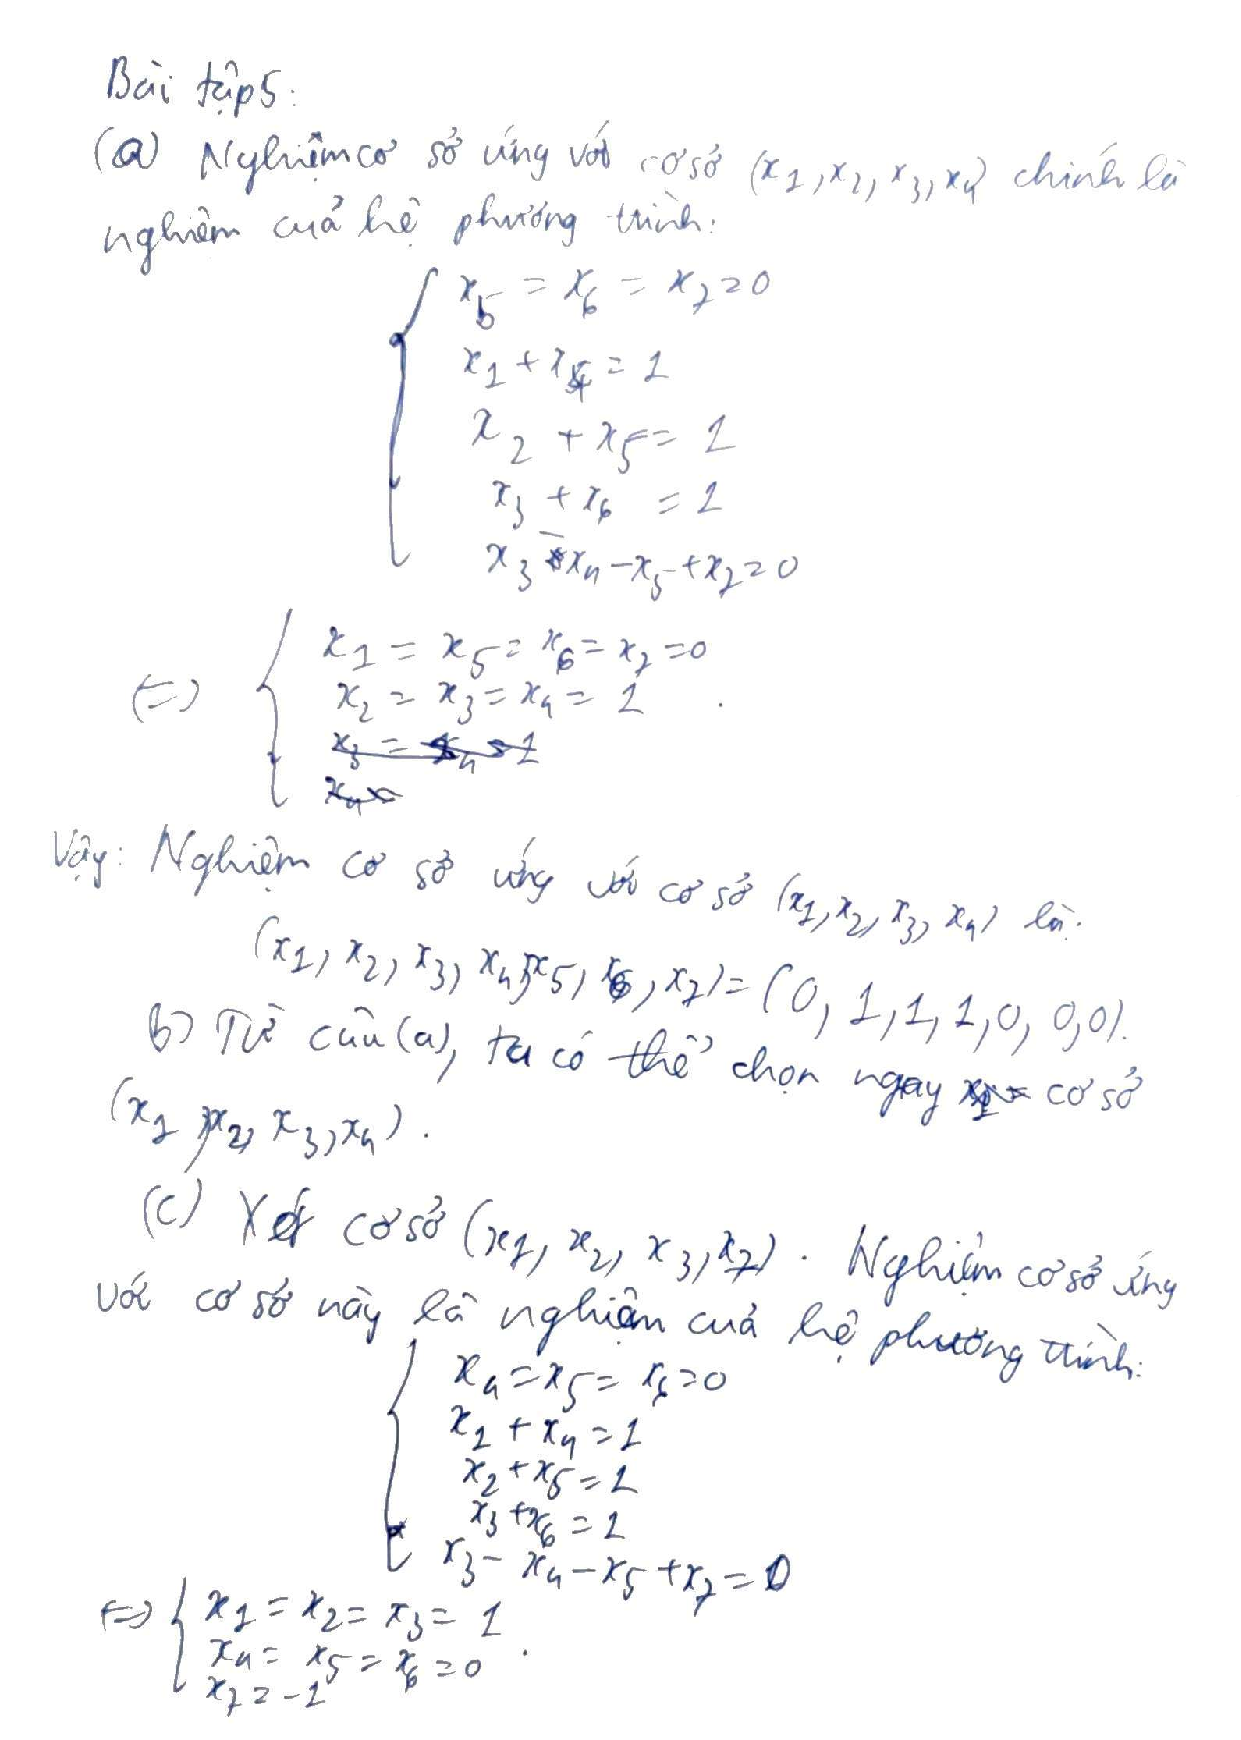
\includepdf[pages=-]{Bai 5(đã sửa)}

\end{document}